\documentclass[a4paper,11pt,cours]{nsi} % COMPILE WITH DRAFT
\geometry{margin=2cm}
\usepackage{hyperref}
\usepackage{yhmath}

\begin{document}

\setcounter{chapter}{8} % 1 de moins que le num de chapitre

\chapter{Probabilités}
\section{Variables aléatoires}
\begin{definition}[ : variable aléatoire]
	Soit $\Omega$ l'univers associé à une expérience aléatoire ($\Omega$ est l'ensemble des issues de l'expérience aléatoire).\\
	On appelle \textbf{variable aléatoire} sur $\Omega$ toute fonction $X$ de $\Omega$ dans $\R$.
\end{definition}

\begin{remarque}[s]
	\begin{enumerate}[label=\textbullet]
		\item 		L'ensemble des valeurs prises par $X$ se note $X(\Omega)=\{x_1 \ ; \ x_2 \ ; \ \ldots \ ; \ x_n\}$.
		\item 		L'évènement « $X$ prend la valeur $x_i$ » se note « $X=x_i$ », il est constitué de tous les éléments de $\Omega$ qui 
		ont 
		pour 								image $x_i$ par la fonction $X$.
	\end{enumerate}
\end{remarque}

\begin{exemple}[]
	On lance deux fois de suite une pièce de monnaie équilibrée et l'on note, après chaque lancer, le côté sorti (P pour Pile, F pour Face). 
	L'ensemble des issues est: $\Omega=\{PP \ ; \ PF \ ; \ FP \ ; \ FF\}$.\\
	On définit un jeu qui consiste à gagner $3$ € à chaque fois que Pile sort et à perdre $2$ € à chaque fois que Face sort.\\
	On définit ainsi une variable aléatoire $X$ sur $\Omega$ qui, à chaque résultat de l'univers, associe le gain relatif (positif ou négatif):
	\begin{enumerate}[label=\textbullet]
		\item 	au résultat $PP$ est associé $6$ €.
		\item 	au résultat $PF$ est associé $1$ €.
		\item 	au résultat $FP$ est associé $1$ €.
		\item 	au résultat $FF$ est associé $-4$ €.
	\end{enumerate}			
	Ainsi $X(\Omega)=\{-4 \ ; \ 1 \ ; \ 6\}$.\\
	L'évènement « $X=1$ » est $\{PF \ ; \ FP\}$.
	Et c\ae tera.
\end{exemple}

\begin{exercice}[ ]
	Un restaurant propose trois menus dont les prix respectifs sont 10 €, 12 € et 18 €. Il y a actuellement 100 clients dans le restaurant.
	\begin{enumerate}
		\item 	On choisit une personne au hasard dans ce restaurant et on lui demande le prix de son menu. Quelle variable aléatoire peut-on définir ici ?\\[0.5em]
		\carreauxseyes{16}{4}
		\item 	On choisit un menu au hasard et on s'intéresse au nombre de personnes dans le restaurant ayant choisi ce menu. Quelle variable aléatoire peut-on définir ici ?\\[0.5em]
		\carreauxseyes{16}{4}
	\end{enumerate}
\end{exercice}
\begin{definition}[ : loi de probabilité d'une variable aléatoire]
	Lorsqu'on associe à chaque valeur $x_i$ de $X(\Omega)$ la probabilité $p_i$ de l'évènement « $X=x_i$ », on définit une loi de probabilité sur 
	$X(\Omega)$. Cette loi est appelée 
	\textbf{{\boldmath loi de probabilité de la variable aléatoire $X$}}.
\end{definition}

\begin{remarque}[]
	On représente souvent la loi de probabilité de la variable aléatoire $X$ à l'aide d'un tableau:
	\begin{center}
		\colorbox{white}{
			\begin{tabular}{|l|c|c|c|c|}
				\hline
				\textbf{{\boldmath Valeur de $X$}} & $x_1$ & $x_2$ & $\cdots$ & $x_n$\\
				\hline
				{\boldmath $P(X=x_i)$} & $p_1$ & $p_2$ & $\cdots$ & $p_n$\\
				\hline
		\end{tabular}}
	\end{center}
	On a: {\boldmath $P(X=x_1)+P(X=x_2)+ \ldots +P(X=x_n)=1$}.
\end{remarque}

\begin{exemple}[]
	Dans l'exemple précédent:
	\begin{enumerate}[label=\textbullet]
		\item 		la probabilité de l'évènement « $X=-4$ » est la probabilité de l'évènement $\{FF\}$:
		\begin{tabbing}
			$P(X=-4)$	\= 	$=P(FF)$	\\[0.5em]
			\>		$=\dfrac{1}{2}\times\dfrac{1}{2}$	\\[0.5em]		
			\>		$=\dfrac{1}{4}$
		\end{tabbing}
		\item 		la probabilité de l'évènement « $X=1$ » est la somme des probabilités des issues $PF$ et $FP$:
		\begin{tabbing}
			$P(X=1)$		\= 	$=P(PF)+P(FP)$	\\[0.5em]
			\>		$=\dfrac{1}{2}\times\dfrac{1}{2}+\dfrac{1}{2}\times\dfrac{1}{2}$	\\[0.5em]
			\>		$=\dfrac{1}{4}+\dfrac{1}{4}$\\[0.5em]
			\>		$=\dfrac{1}{2}$
		\end{tabbing}
		\item 		la probabilité de l'évènement « $X=6$ » est la probabilité de l'évènement $\{PP\}$: 
		
		$P(X=6)=\dfrac{1}{4}$.
	\end{enumerate}			
	
	La loi de probabilité de la variable aléatoire $X$ est résumée dans le tableau ci-dessous:
	\begin{center}
		\colorbox{white}{
			\begin{tabular}{|c|c|c|c|}
				\hline
				{\boldmath $x_i$} & $-4$ & $1$ & $6$ \\
				\hline
				& & & \\
				{\boldmath $P(X=x_i)$} & $\dfrac{1}{4}$ & $\dfrac{1}{2}$ & $\dfrac{1}{4}$\\
				& & & \\			
				\hline
		\end{tabular}}
	\end{center}
\end{exemple}



\section{Espérance, variance et écart-type}
\begin{definition}[ : espérance, variance et écart-type]
	Soit $X$ une variable aléatoire dont la loi de probabilité est résumée dans le tableau ci-dessous:
	\begin{center}
		\colorbox{white}{
			\begin{tabular}{|l|c|c|c|c|}
				\hline
				\textbf{{\boldmath Valeur de $X$}} & $x_1$ & $x_2$ & $\cdots$ & $x_n$\\
				\hline
				{\boldmath $P(X=x_i)$} & $p_1$ & $p_2$ & $\cdots$ & $p_n$\\
				\hline
		\end{tabular}}
	\end{center}
	
	\begin{enumerate}[label=\textbullet]
		\item	L'\textbf{{\boldmath espérance de $X$}} est le nombre noté {\boldmath $E(X)$} défini par:\\
		\centerline{{\boldmath $E(X)=p_1 x_1+p_2 x_2+\ldots+p_n x_n$}} 
		noté aussi {\boldmath $E(X)=\displaystyle \sum_{i=1}^{n} p_i x_i$}.
		\item La 	\textbf{{\boldmath variance de $X$}} le nombre noté {\boldmath $V(X)$} défini par:\\
		\centerline{{\boldmath $V(X)=p_1 \left(x_1-E(X)\right)^2+p_2 \left(x_2-E(X)\right)^2+\ldots+p_n \left(x_n-E(X)\right)^2$}}
		noté aussi {\boldmath $V(x)=\displaystyle \sum_{i=1}^{n} p_i\left(x_i-E(X)\right)^2$}.
		\item  L'\textbf{{\boldmath écart-type de $X$}} le nombre noté {\boldmath $\sigma(X)$} défini par: {\boldmath $\sigma(X)=\sqrt{V(X)}$}.
	\end{enumerate}
\end{definition}

\begin{exemple}[]
	Dans l'exemple précédent la loi de probabilité de la variable aléatoire $X$ est résumée dans le tableau ci-dessous:
	\begin{center}
		\colorbox{white}{
			\begin{tabular}{|c|c|c|c|}
				\hline
				{\boldmath $x_i$} & $-4$ & $1$ & $6$ \\
				\hline
				& & & \\
				{\boldmath $P(X=x_i)$} & $\dfrac{1}{4}$ & $\dfrac{1}{2}$ & $\dfrac{1}{4}$\\
				& & & \\
				\hline
		\end{tabular}}
	\end{center}
	\begin{multicols}{2}
		\begin{tabbing}
			$E(X)$	\=	$=\dfrac{1}{4}\times(-4)+\dfrac{1}{2}\times1+\dfrac{1}{4}\times 6$\\[0.5em]
			\>	$=-1+\dfrac{1}{2}+\dfrac{3}{2}$\\[0.5em]
			\>	$=-1+\dfrac{4}{2}$\\[0.5em]
			\>	$=-1+2$\\[0.5em]
			\>	$=1$
		\end{tabbing}
		\columnbreak
		\begin{tabbing}
			$V(X)$	\=	$=\dfrac{1}{4}(-4-1)^2+\dfrac{1}{2}(1-1)^2+\dfrac{1}{4}(6-1)^2$\\[0.5em]
			\>	$=\dfrac{1}{4}\times(-5)^2+0+\dfrac{1}{4}\times5^2$\\[0.5em]
			\>	$=\dfrac{25}{4}+\dfrac{25}{4}$\\[0.5em]
			\>	$=\dfrac{25}{2}$\\[0.5em]
			\>	$=12,5$
		\end{tabbing}
	\end{multicols}
	Ainsi
	\begin{tabbing}
		$\qquad\sigma(X)$	\=	$=\sqrt{V(X)}$\\[0.5em]
		\>	$=\sqrt{12,5}$\\[0.5em]
		\>	$ \approx 3,5$.
	\end{tabbing}
\end{exemple}

\begin{propriete}[]
	\begin{enumerate}[label=\textbullet]
		\item 	On a aussi: {\boldmath $V(X)=E(X^2)-[E(X)]^2$}.
		\item 	Soit $a$ et $b$ deux réels. Alors: {\boldmath $\quad E(aX+b)=aE(X)+b\quad$ et 							$\quad V(aX)=a^2 V(X)$}.
	\end{enumerate}
\end{propriete}

\begin{demonstration}
	\begin{enumerate}[label=\textbullet]
		\item 	\begin{tabbing}
			$V(X)$	\=$=\displaystyle \sum_{i=1}^{n} p_i\left(x_i-E(X)\right)^2$\\[0.5em]
			\>$=\displaystyle \sum_{i=1}^{n} \left(p_i x_i^2-2p_i x_i E(X)+p_i E(X)^2\right)$\\[0.5em]
			\>$=\displaystyle \sum_{i=1}^{n} p_i x_i^2-2E(X)\displaystyle 			\sum_{i=1}^{n} p_i 
			x_i+E(X)^2\displaystyle \sum_{i=1}^{n} p_i$\\[0.5em]
			\>$=E(X^2)-2E(X)\times E(X)+E(X)^2\times1$\\[0.5em]
			\>$=E(X^2)-2E(X)^2+E(X)^2$\\[0.5em]
			\>$=E(X^2)-E(X)^2$
		\end{tabbing}

		\item 	Lois de probabilités des variables aléatoires $aX$ et $aX+b$:
		\begin{center}
			\colorbox{white}{
				\begin{tabular}{|l|c|c|c|c|}
					\hline
					{\boldmath $X$} & $x_1$ & $x_2$ & $\cdots$ & $x_n$\\
					\hline
					{\boldmath $aX$} & $ax_1$ & $ax_2$ & $\cdots$ & $ax_n$\\
					\hline
					{\boldmath $aX+b$} & $ax_1+b$ & $ax_2+b$ & $\cdots$ & $ax_n+b$\\
					\hline
					\textbf{Probabilité} & $p_1$ & $p_2$ & $\cdots$ & $p_n$\\
					\hline
			\end{tabular}}
		\end{center}
		\begin{tabbing}
			$E(aX+b)$	\=	$=p_1(ax_1+b)+p_2(ax_2+b)+\ldots+p_n(ax_n+b)$\\[0.5em]
			\>$=a(p_1x_1+p_2x_2+\ldots+p_n x_n)+b(p_1+p_2+\ldots+p_n)$\\[0.5em]
			\>$=aE(X)+b\quad$  puisque l'on a $\quad p_1+p_2+\ldots+p_n=1$
		\end{tabbing}
	\end{enumerate}
	\begin{enumerate}[label=\textbullet]
		\item 	\begin{tabbing}
			$V(aX)$	\=	  $=p_1\left(ax_1-E(aX)\right)^2+p_2\left(ax_2-E(aX)\right)^2+\ldots+p_n\left(ax_n-E(aX)\right)^2$\\[0.5em]
			\>$=a^2p_1\left(x_1-E(X)\right)^2+a^2p_2\left(x_2-E(X)\right)^2+\ldots+a^2p_n\left(x_n-E(X)\right)^2$\\[0.5em]
			\>$=a^2\left[p_1\left(x_1-E(X)\right)^2+p_2\left(x_2-E(X)\right)^2+\ldots+p_n\left(x_n-E(X)\right)^2\right]$\\[0.5em]
			\>$=a^2V(X)$
		\end{tabbing}
	\end{enumerate}
\end{demonstration}

\subsection*{Interprétation de l'espérance et de l'écart-type}
Lors d'un jeu, l'\textbf{espérance de gain} représente le \textbf{gain moyen} que peut espérer le joueur lors d'un grand nombre de parties.
\begin{itemize}
	\item 	Si ce gain moyen est \textbf{nul}, on dit que le jeu est \textbf{équitable}.
	\item 	Si ce gain moyen est \textbf{positif}, on dit que le jeu est \textbf{favorable} au joueur
	\item 	Si ce gain moyen est \textbf{négatif}, on dit que le jeu est \textbf{défavorable} au joueur.
\end{itemize}
L'\textbf{écart-type du gain} mesure la \textbf{dispersion} des gains autour du gain moyen.\\
Plus l'écart-type est grand, plus la variable aléatoire est dispersée et plus le degré de risque du jeu est grand.

\section{Répétition d'expériences identiques et indépendantes}

\begin{definition}[ : Expériences indépendantes]
	On considère $n$ expériences aléatoires \textbf{identiques} successives. Si les résultats de chacune d'elles ne dépendent pas des résultats 
	des expériences précédentes, on dit que ces expériences sont \textbf{indépendantes}.
\end{definition}

\begin{exemple}[]
	Une urne contient $4$ boules bleues, $3$ boules noires et $2$ boules vertes. 
	On tire successivement deux boules \textbf{avec remise}. Il s'agit donc d'une répétition de deux expériences identiques et indépendantes.
\end{exemple}

\subsection*{Modélisation à l'aide d'un arbre pondéré}
Dans l'exemple précédent, la répétition des deux expériences peut être représentée par un arbre pondéré:
\begin{center}
	% Racine à Gauche, développement vers la droite
	\begin{tikzpicture}[xscale=1,yscale=.7]
		% Styles (MODIFIABLES)
		\tikzstyle{fleche}=[-,thick]
		\tikzstyle{noeud}=[fill=yellow,circle,draw]
		\tikzstyle{noeudB}=[fill=blue!50,circle,draw]
		\tikzstyle{noeudN}=[fill=gray!50,circle,draw]
		\tikzstyle{noeudV}=[fill=green!50,circle,draw]
		\tikzstyle{feuille}=[fill=yellow!50,circle,draw]
		\tikzstyle{feuilleB}=[fill=blue!50,circle,draw]
		\tikzstyle{feuilleN}=[fill=gray!50,circle,draw]
		\tikzstyle{feuilleV}=[fill=green!50,circle,draw]
		\tikzstyle{etiquette}=[midway,below]
		% Dimensions (MODIFIABLES)
		\def\DistanceInterNiveaux{3}
		\def\DistanceInterFeuilles{2}
		% Dimensions calculées (NON MODIFIABLES)
		\def\NiveauA{(0)*\DistanceInterNiveaux}
		\def\NiveauB{(1.5)*\DistanceInterNiveaux}
		\def\NiveauC{(2.5)*\DistanceInterNiveaux}
		\def\InterFeuilles{(-1)*\DistanceInterFeuilles}
		% Noeuds (MODIFIABLES : Styles et Coefficients d'InterFeuilles)
		\node[noeud] (R) at ({\NiveauA},{(4)*\InterFeuilles}) {$ $};
		\node[noeudB] (Ra) at ({\NiveauB},{(1)*\InterFeuilles}) {$B$};
		\node[feuilleB] (Raa) at ({\NiveauC},{(0)*\InterFeuilles}) {$B$};
		\node[feuilleN] (Rab) at ({\NiveauC},{(1)*\InterFeuilles}) {$N$};
		\node[feuilleV] (Rac) at ({\NiveauC},{(2)*\InterFeuilles}) {$V$};
		\node[noeudN] (Rb) at ({\NiveauB},{(4)*\InterFeuilles}) {$N$};
		\node[feuilleB] (Rba) at ({\NiveauC},{(3)*\InterFeuilles}) {$B$};
		\node[feuilleN] (Rbb) at ({\NiveauC},{(4)*\InterFeuilles}) {$N$};
		\node[feuilleV] (Rbc) at ({\NiveauC},{(5)*\InterFeuilles}) {$V$};
		\node[noeudV] (Rc) at ({\NiveauB},{(7)*\InterFeuilles}) {$V$};
		\node[feuilleB] (Rca) at ({\NiveauC},{(6)*\InterFeuilles}) {$B$};
		\node[feuilleN] (Rcb) at ({\NiveauC},{(7)*\InterFeuilles}) {$N$};
		\node[feuilleV] (Rcc) at ({\NiveauC},{(8)*\InterFeuilles}) {$V$};
		% Arcs (MODIFIABLES : Styles)
		\draw[fleche] (R)--(Ra) node[etiquette] {\tiny$\dfrac{4}{9}$};
		\draw[fleche] (Ra)--(Raa) node[etiquette] {\tiny$\dfrac{4}{9}$};
		\draw[fleche] (Ra)--(Rab) node[etiquette] {\tiny$\dfrac{3}{9}$};
		\draw[fleche] (Ra)--(Rac) node[etiquette] {\tiny$\dfrac{2}{9}$};
		\draw[fleche] (R)--(Rb) node[etiquette] {\tiny$\dfrac{3}{9}$};
		\draw[fleche] (Rb)--(Rba) node[etiquette] {\tiny$\dfrac{4}{9}$};
		\draw[fleche] (Rb)--(Rbb) node[etiquette] {\tiny$\dfrac{3}{9}$};
		\draw[fleche] (Rb)--(Rbc) node[etiquette] {\tiny$\dfrac{2}{9}$};
		\draw[fleche] (R)--(Rc) node[etiquette] {\tiny$\dfrac{2}{9}$};
		\draw[fleche] (Rc)--(Rca) node[etiquette] {\tiny$\dfrac{4}{9}$};
		\draw[fleche] (Rc)--(Rcb) node[etiquette] {\tiny$\dfrac{3}{9}$};
		\draw[fleche] (Rc)--(Rcc) node[etiquette] {\tiny$\dfrac{2}{9}$};
	\end{tikzpicture}
\end{center}	


	
%\begin{minipage}{6cm}
%	\includegraphics{fig2.eps}
%\end{minipage}
L'univers de cette expérience aléatoire se compose de $9$ couples de résultats correspondants chacun aux $9$ chemins de l'arbre:\\
On fait l'abus de notation consistant à noter par exemple $BB$ à la place du couple $(B;B)$ :\\
$\Omega=\left\{BB\ ;\ BN\ ;\ BV\ ;\ NB\ ; \ NN \ ; \ NV \ ; \ VB \ ; \ VN \ ; \ VV\right\}$.\\
\begin{propriete}[ : choix d'une loi de probabilité]
	Dans le cas d'une répétition d'expériences identiques et indépendantes représentée par un arbre pondéré:\\
	- La probabilité d'un évènement correspondant à un chemin sur l'arbre est obtenue en multipliant les probabilités portées par les branches.\\
	- La probabilité d'un évènement correspondant à plusieurs chemins est alors obtenue en ajoutant les probabilités des évènements 
	correspondants à chaque chemin, puisque ceux-ci sont incompatibles.
\end{propriete}

\begin{exemple}[]
	Dans l'exemple précédent:\\
	- La probabilité d'obtenir le couple $VN$ est égale au produit $\dfrac{2}{9}\times\dfrac{3}{9}=\dfrac{6}{81}=\dfrac{2}{27}$.\\
	
	- Si l'on considère l'évènement $A$: « obtenir au moins une boule noire », alors $A=\{BN;NB;NN;NV;VN\}$. Alors 
	\begin{tabbing}
		$P(A)$	\=$=P(BN)+P(NN)+P(VN)$\\[0.5em]
		\>$=\dfrac{4}{9}\times\dfrac{3}{9}+\dfrac{1}{3}+\dfrac{2}{9}\times\dfrac{3}{9}$\\[0.5em]
		\>$=\dfrac{12}{81}+\dfrac{27}{81}+\dfrac{6}{81}$\\[0.5em]
		\>$=\dfrac{45}{81}$\\[0.5em]	
		\>$=\dfrac{5}{9}$
	\end{tabbing}
\end{exemple}

\section{L'essentiel du chapitre}
\begin{aretenir}
	\begin{center}
		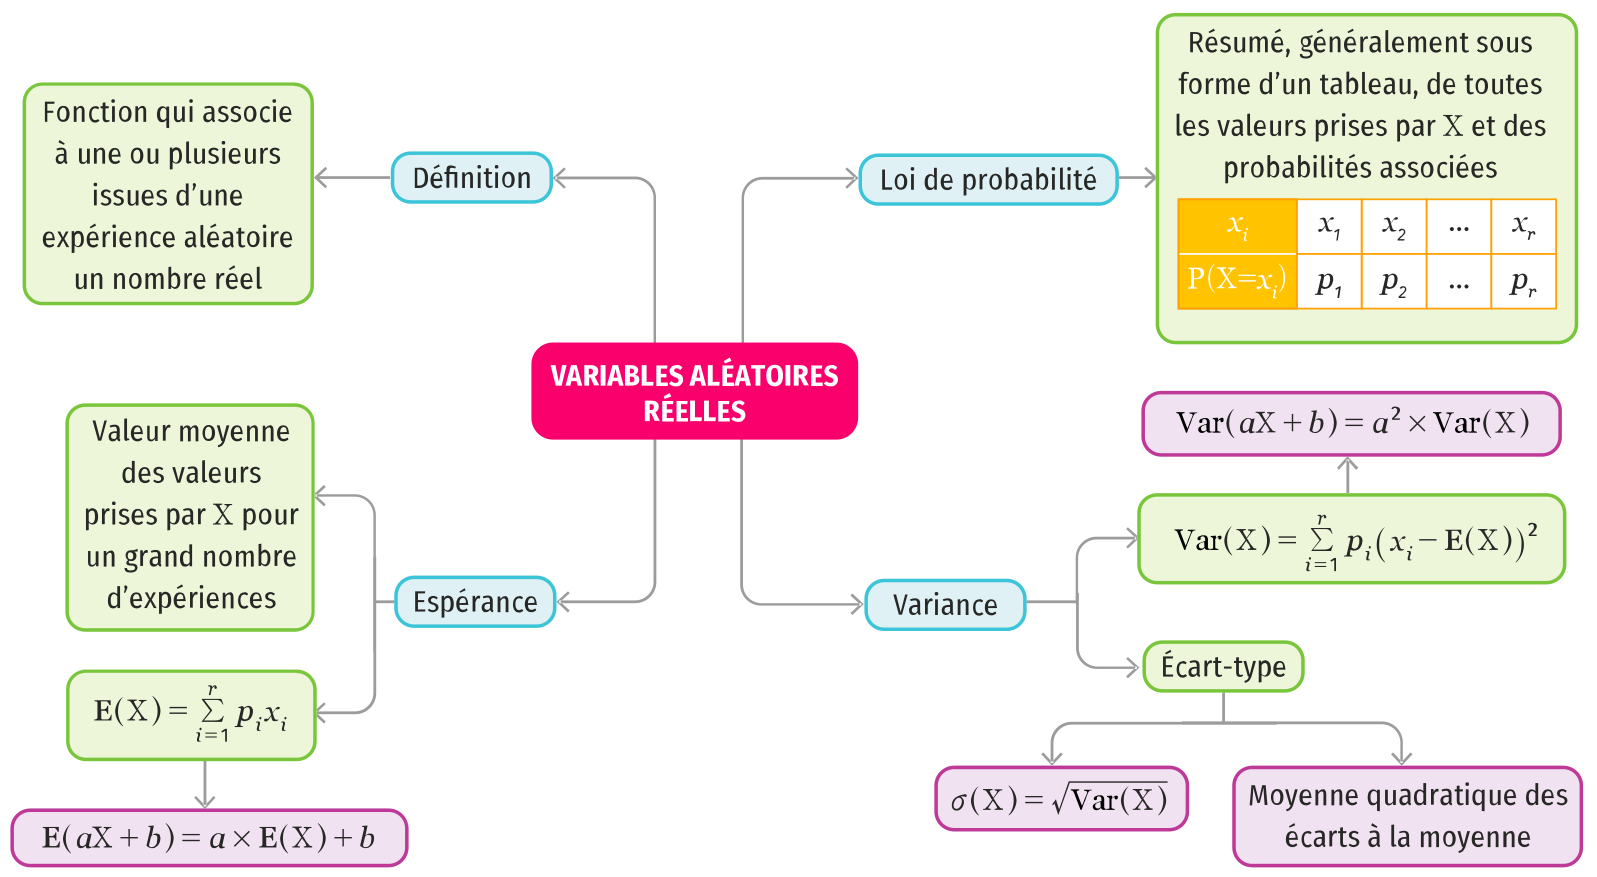
\includegraphics[width=16cm]{aretenir}
	\end{center}
\end{aretenir}
\end{document}
